\begin{figure}[tbp]\centering
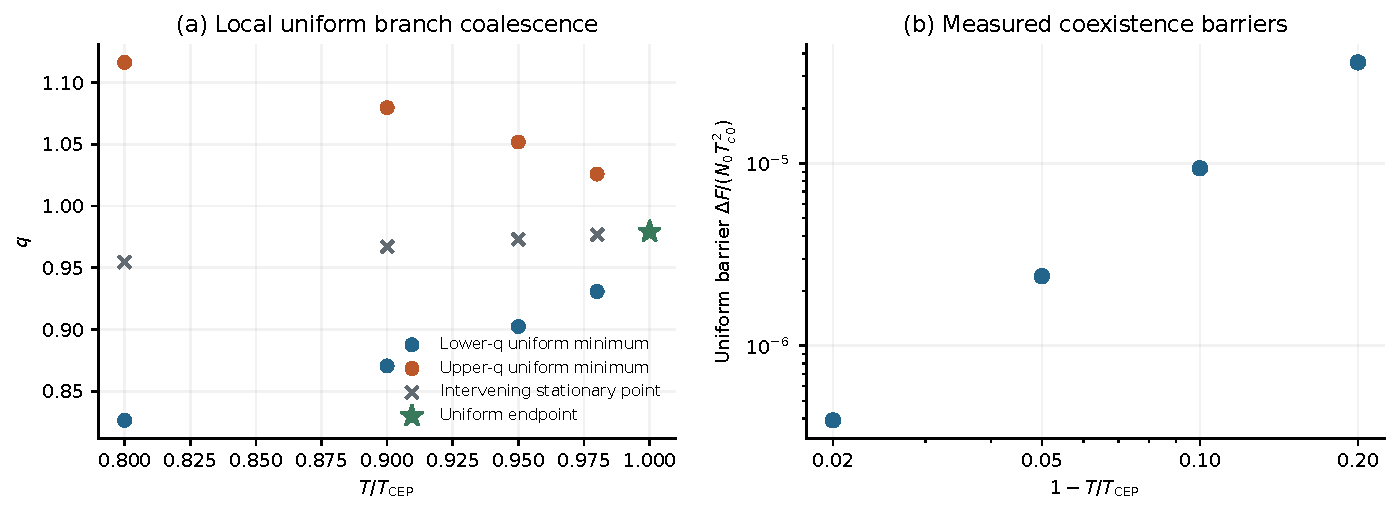
\includegraphics[width=\textwidth]{figures/fig01_endpoint_topology.pdf}
\caption{Restricted uniform endpoint topology. Samples at four temperatures between $0.80T_*$ and $0.98T_*$ show the two coexistence minima and intervening stationary point; the right panel gives uniform barriers. The field varies along coexistence, and connecting samples does not establish a fixed-field scan or fitted critical law.}\label{fig:endpoint}
\end{figure}
\begin{figure}[tbp]\centering
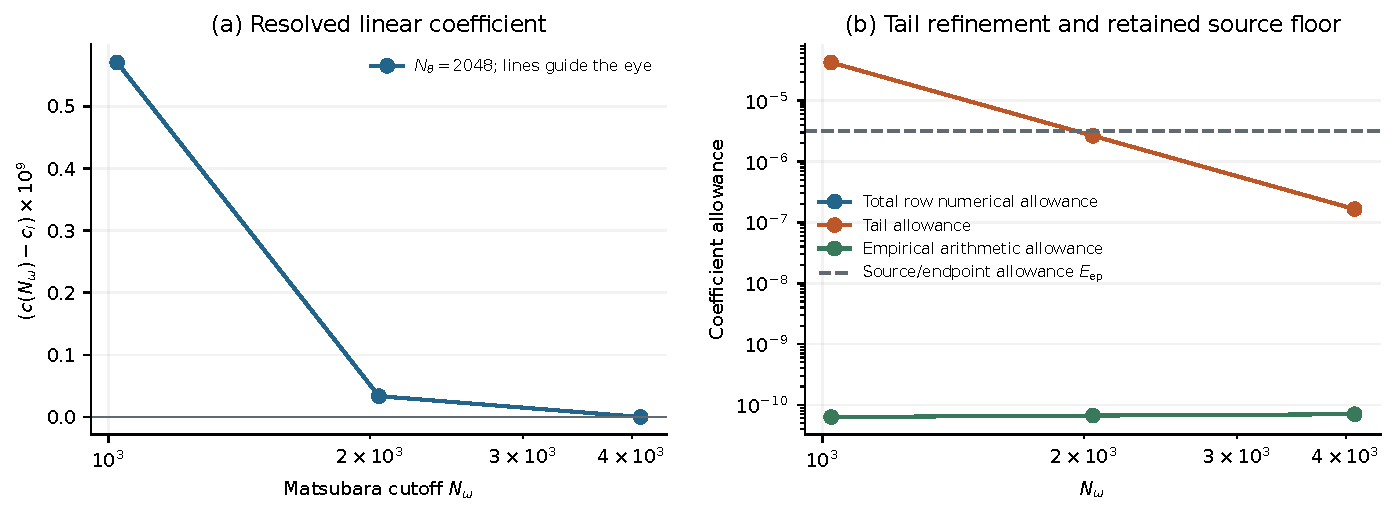
\includegraphics[width=\textwidth]{figures/fig02_linear_qualification.pdf}
\caption{Second quadratic-response representation under frequency refinement at $N_\theta=2048$. Coefficients are measured relative to the finest row; the right panel separates row numerical, tail, and primitive-arithmetic radii from the endpoint allowance. The final allowance also includes single- and mixed-refinement contributions.}\label{fig:linear}
\end{figure}
\begin{figure}[tbp]\centering
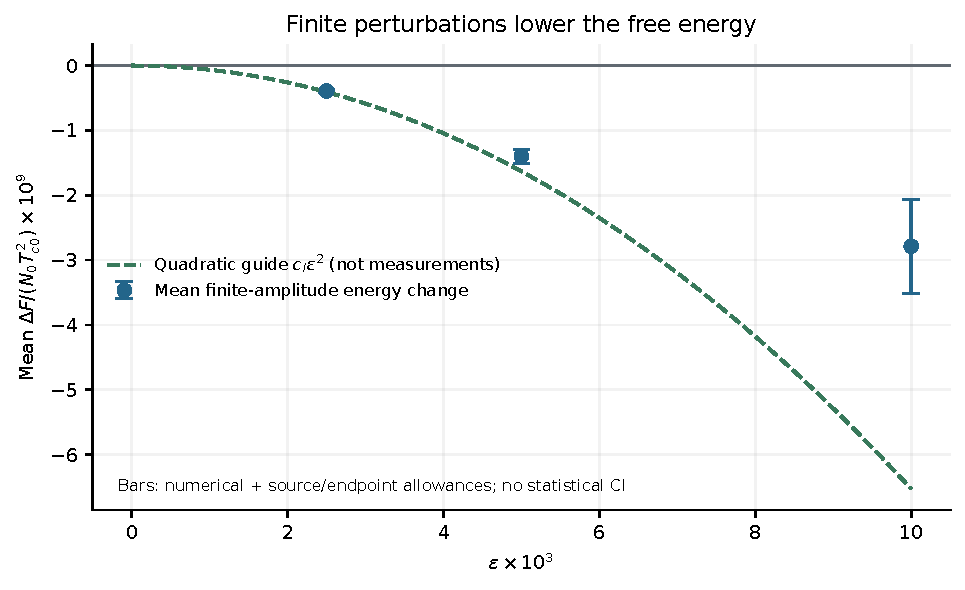
\includegraphics[width=\textwidth]{figures/fig04_energy_descent.pdf}
\caption{Paired mean energy change $\overline{\delta f}=\epsilon^2C$ in units of $N_0\Tc^2$, reconstructed from the computed quotients with radius $\epsilon^2(E_C+E_{\mathrm{ep}})$. The dashed $\cI\epsilon^2$ curve is a quadratic guide. A negative paired mean ensures a descending signed member without assigning equal lowering to both signs.}\label{fig:energy}
\end{figure}
\begin{figure}[tbp]\centering
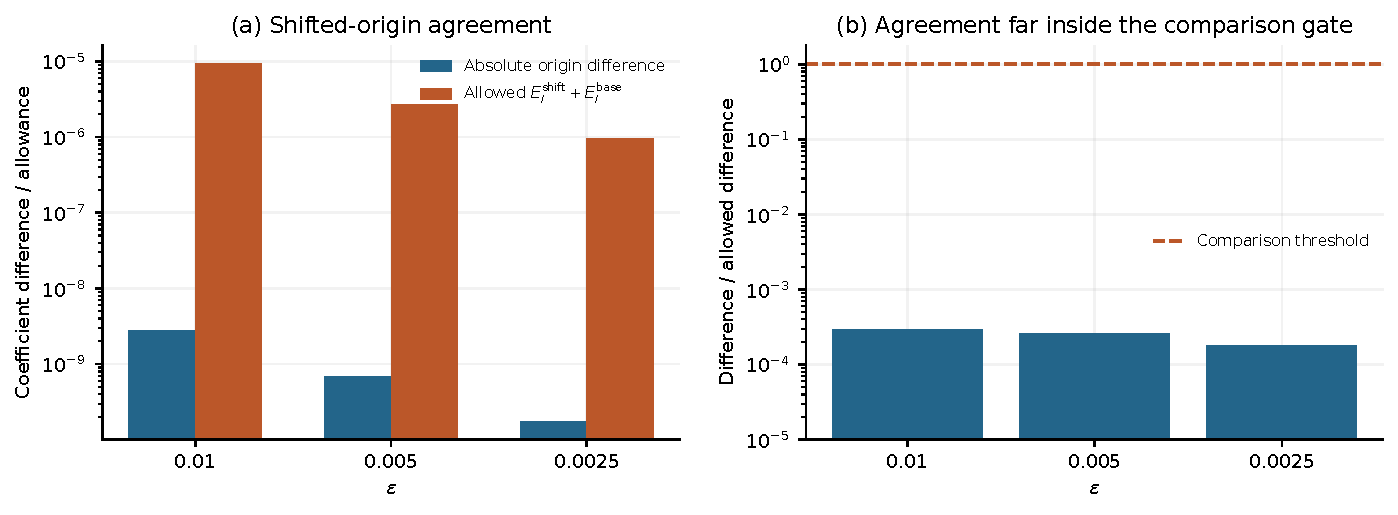
\includegraphics[width=\textwidth]{figures/fig05_origin_agreement.pdf}
\caption{Angular-origin sensitivity. Absolute quotient differences after shifting the origin by $\pi\sqrt5/256$ are smaller than the sum of complete numerical allowances. The comparison shares the physical direction, linear baseline, and domain estimates; common endpoint uncertainty is excluded from the difference allowance.}\label{fig:origin}
\end{figure}
\begin{figure}[tbp]\centering
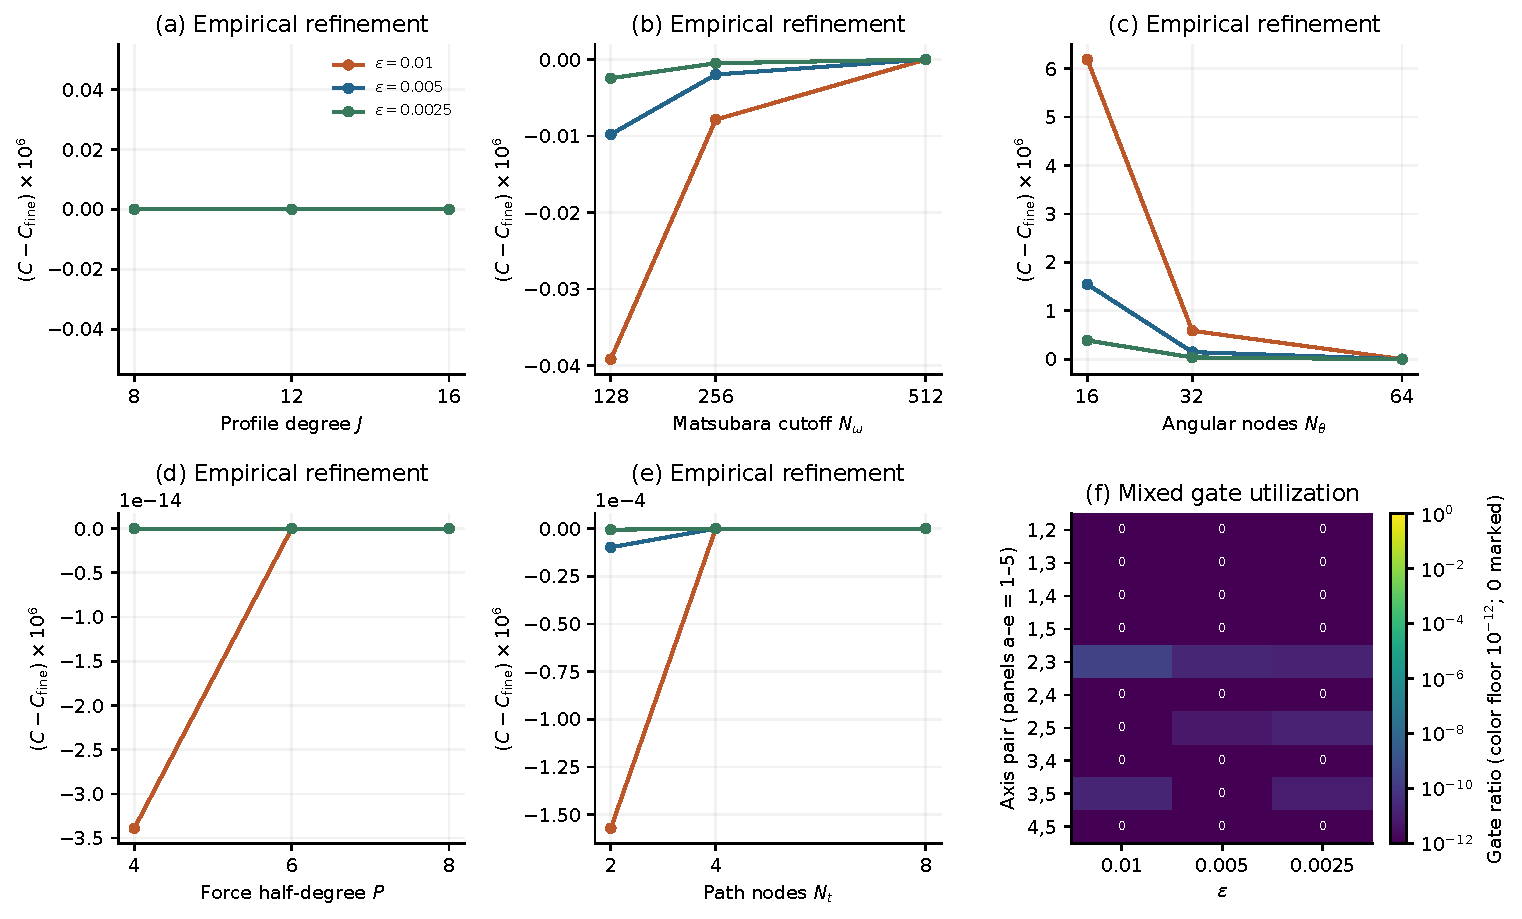
\includegraphics[width=\textwidth]{figures/fig06_axis_mixed_convergence.pdf}
\caption{Single- and mixed-refinement diagnostics. Single-axis changes relative to the finest row are shown in units of $10^{-6}$, with axis definitions in Table~\ref{tab:levels}. The final panel gives the larger utilization of the two inequalities in Appendix~\ref{app:errors}; values below $10^{-12}$ share the lowest colour, and computed exact zeros are marked.}\label{fig:axes}
\end{figure}
\FloatBarrier
